\documentclass[conference]{IEEEtran}
\usepackage[utf8]{inputenc}
\usepackage[T1]{fontenc}
\usepackage[spanish]{babel}
\usepackage{amsmath,amssymb}
\usepackage{graphicx}
\usepackage{tabularx}
\usepackage{booktabs}
\usepackage{array}
\usepackage{xurl}
\usepackage[hidelinks]{hyperref}
\usepackage{multirow}
\usepackage{csquotes}
\usepackage{cite}
\usepackage{caption}
\usepackage{float}

\addto\captionsspanish{
  \renewcommand{\figurename}{Figura}
  \renewcommand{\tablename}{Tabla}
  \renewcommand{\appendixname}{Anexo}
}

\renewcommand{\thesection}{\arabic{section}}
\renewcommand{\thesubsection}{\thesection.\arabic{subsection}}
\renewcommand{\thesubsubsection}{\thesubsection.\arabic{subsubsection}}
\renewcommand{\thetable}{\arabic{table}}

\title{Refinamiento empírico de constructos cualitativos: un enfoque de métodos mixtos con modelos SEM asistidos por LLM en la educación virtual postpandemia}

\author{}
\date{}

\begin{document}
\raggedbottom % Para controlar el espacio extra entre párrafos

\maketitle

\begin{abstract}
La transición forzada hacia la educación virtual universitaria tras la pandemia de COVID-19 transformó profundamente la experiencia estudiantil, demandando enfoques de métodos mixtos que combinen la riqueza de las vivencias subjetivas con la solidez de la evidencia cuantitativa. Sin embargo, la integración entre ambas fases suele limitarse a una descripción narrativa, lo que dificulta la validación y el refinamiento formal de los constructos cualitativos y puede derivar en especificaciones estructurales con un ajuste o una fiabilidad subóptimos. Para resolver este desafío, se desarrolló un diseño secuencial exploratorio en la Universidad de Cuenca mediante un cuestionario aplicado a 513 estudiantes, construido sobre un marco cualitativo previo de 6 temas y 26 códigos. La integración de análisis exploratorio, clustering y análisis factorial exploratorio generó insumos para que modelos de inteligencia artificial (Gemini y DeepSeek) propusieran variables latentes y modelos de ecuaciones estructurales (SEM), evaluados posteriormente con análisis factorial confirmatorio. El modelo generado por DeepSeek con datos agrupados alcanzó un ajuste sobresaliente ($\text{CFI} = 0.9953$, $\text{RMSEA} = 0.0177$), superando la especificación cualitativa original. Además, los hallazgos permitieron refinar el marco conceptual al corroborar la bidimensionalidad emocional, diferenciar la selección del uso de herramientas de IA y separar los problemas técnicos de los factores de distracción. Este trabajo demuestra una ruta para validar y enriquecer constructos cualitativos mediante la articulación auténtica de métodos mixtos e inteligencia artificial. 
\end{abstract}

\noindent\textbf{Keywords:} Modelos de ecuaciones estructurales, métodos mixtos, análisis factorial exploratorio, análisis factorial confirmatorio, clustering.

% ============================================================
\section{Introducción}
\label{sec:introduccion}
% ============================================================

La pandemia de COVID-19 provocó una transformación abrupta de los sistemas educativos a nivel mundial \cite{unesco2021covid}. En Ecuador, las universidades migraron forzosamente hacia modalidades virtuales, generando cambios profundos en las prácticas pedagógicas, las condiciones materiales de estudio y el bienestar psicosocial de los estudiantes \cite{castillosanchezEducacionVirtualImplementada2021}. La Universidad de Cuenca, con miles de estudiantes transitando de la presencialidad a la virtualidad y posteriormente de regreso a las aulas \cite{eluniverso2021retornoUCuenca}, constituye un caso paradigmático para estudiar este fenómeno desde una perspectiva integral.

Abordar un fenómeno de esta complejidad exige estrategias metodológicas que trasciendan los enfoques puramente cuantitativos o cualitativos. Los métodos mixtos, en particular el diseño secuencial exploratorio, ofrecen un marco idóneo al permitir que los hallazgos cualitativos guíen el desarrollo de instrumentos cuantitativos para validar y generalizar los patrones observados \cite{creswellDesigningConductingMixed}. La transición del análisis factorial exploratorio a los modelos de ecuaciones estructurales suele depender de decisiones manuales o heurísticas que pueden comprometer el ajuste. En este contexto, los modelos de lenguaje de gran escala (LLM) pueden facilitar la síntesis de literatura especializada y la traducción de patrones empíricos en constructos y modelos estructurales teóricamente fundamentados.

Este artículo describe el diseño de una investigación que, a partir de un análisis cualitativo previo sobre la experiencia estudiantil durante la educación virtual, desarrolló y aplicó un cuestionario a 513 estudiantes. Los datos recopilados fueron analizados mediante un análisis exploratorio de datos (EDA), técnicas de clustering y análisis factorial exploratorio (AFE) con componentes principales (PCA). Estos resultados empíricos sirvieron de insumo para que modelos LLM asistieran en dos tareas analíticas clave: la interpretación semántica de los perfiles estudiantiles obtenidos por agrupamiento, y la especificación de variables latentes y rutas estructurales fundamentadas en la literatura. Posteriormente, se evaluó la fiabilidad y el ajuste estructural de estos modelos, comparándolos con un modelo original basado en los temas cualitativos y con modelos adicionales derivados de la experimentación, mediante pruebas de análisis factorial confirmatorio (CFA).

Las principales contribuciones de este estudio radican en demostrar que la especificación de modelos de ecuaciones estructurales asistida por LLM a partir de insumos factoriales puede alcanzar un ajuste competitivo y una mayor fiabilidad que los modelos derivados únicamente del análisis cualitativo. Asimismo, este estudio identifica el modelo con las mejores propiedades entre las diferentes especificaciones evaluadas y aporta evidencia empírica que respalda la validez de los constructos latentes (inferidos por inteligencia artificial) en el contexto de la educación virtual posterior a la pandemia. Finalmente, se plantea una estrategia de integración que permite superar la presentación fragmentada de los métodos mixtos, y refinar empíricamente las categorías conceptuales iniciales.

El artículo se estructura en cuatro secciones. Después de esta introducción, la sección~\ref{sec:antecedentes} revisa los antecedentes y trabajos relacionados; la sección~\ref{sec:metodologia} describe el proceso metodológico y presenta los resultados obtenidos; y la sección~\ref{sec:conclusiones} expone las principales conclusiones y las líneas de trabajo futuro.

% ============================================================
\section{Antecedentes y trabajos relacionados}
\label{sec:antecedentes}
% ============================================================
La literatura sobre métodos mixtos, educación virtual en pandemia y técnicas de validación cuantitativa de marcos cualitativos constituye el fundamento teórico y metodológico de esta investigación. A continuación, se revisan los aportes más relevantes en cada una de estas áreas, en trabajos enfocados en América Latina, identificando los vacíos que el presente estudio busca cubrir.

\subsection{Métodos mixtos}

Los métodos mixtos de investigación han ganado un reconocimiento creciente en las ciencias sociales y educativas durante las últimas dos décadas. Creswell y Plano Clark \cite{creswellDesigningConductingMixed} los definen como un enfoque que combina la recolección y el análisis de datos cuantitativos y cualitativos en un mismo estudio, con el propósito de lograr una comprensión más completa del fenómeno investigado que la que proporcionaría cualquiera de los dos enfoques por separado. Esta integración puede adoptar diversas configuraciones según la prioridad relativa de cada componente y la secuencia temporal en que se ejecutan.

Dentro de la taxonomía propuesta por Creswell y Plano Clark, el diseño secuencial exploratorio se caracteriza por iniciar con una fase cualitativa orientada a explorar un fenómeno desde la perspectiva de los participantes, cuyos resultados guían el desarrollo de instrumentos cuantitativos aplicados en una segunda fase. Este diseño resulta particularmente apropiado cuando no existen instrumentos validados para medir los constructos de interés o cuando se desea que la operacionalización de las variables esté arraigada en el lenguaje y las experiencias reales de los sujetos de estudio \cite{creswellDesigningConductingMixed} \cite{tashakkoriFoundationsMixedMethods2021}.

La fortaleza del diseño secuencial exploratorio radica en que la fase cualitativa dota de validez convergente al instrumento cuantitativo, mientras que la fase cuantitativa permite evaluar la generalizabilidad de los hallazgos cualitativos. Esta complementariedad resulta especialmente valiosa en contextos educativos donde las vivencias subjetivas como las emociones, las percepciones sobre la calidad docente o las dificultades de aprendizaje requieren ser capturadas primero en profundidad y luego cuantificadas para identificar patrones poblacionales.

No obstante, este diseño también enfrenta desafíos metodológicos significativos. El principal reside en la integración de los resultados de ambas fases, una etapa que con frecuencia se reduce a una yuxtaposición narrativa carente de un procedimiento sistemático de contrastación. Como señalan Fetters et al. \cite{fettersAchievingIntegrationMixed2013}, la verdadera integración ocurre cuando los hallazgos de un componente se utilizan activamente para informar, validar o refinar los del otro, más allá de su mera presentación secuencial.

\subsection{Modelos de Ecuaciones Estructurales y Análisis Factoriales}
Los Modelos de Ecuaciones Estructurales (SEM) representan un conjunto de técnicas estadísticas diseñadas para estimar la magnitud y la dirección de supuestos efectos causales en estudios cuantitativos \cite{kline2023principles}. Estas técnicas permiten integrar el análisis de regresión con el análisis factorial, facilitando el análisis de relaciones no solo entre variables observadas, sino también entre constructos latentes o teóricos que no se miden directamente. El objetivo central del SEM es poner a prueba teorías mediante la especificación de modelos que representan predicciones teóricas, evaluando qué tan bien se ajustan estos modelos a los datos empíricos recolectados.

El Análisis Factorial Exploratorio (AFE) es una técnica que se utiliza principalmente en las etapas iniciales de una investigación o cuando la teoría sobre cómo se miden ciertos conceptos aún es débil o está en desarrollo \cite{kline2023principles}. A diferencia de otros métodos, el AFE analiza modelos de medición no restringidos, lo que significa que permite que cada indicador o ítem cargue sobre todos los factores identificados, dejando que los propios datos revelen la estructura subyacente que lleva a la identificación de constructos o variables latentes que no se pueden medir directamente.

En contraste, el Análisis Factorial Confirmatorio (CFA) es una técnica verificadora que se emplea para evaluar si una estructura que involucra variables latentes, variables observadas y las relaciones entre ellas, se ajusta adecuadamente a los datos observados \cite{kline2023principles}. En el CFA, el investigador especifica de antemano el número exacto de variables y las relaciones precisas entre ellas. Este enfoque es esencialmente confirmatorio, ya que permite poner a prueba hipótesis específicas sobre la validez de constructo y asegurar que los indicadores midan fielmente las variables latentes según lo previsto por la teoría.

\subsection{Trabajos relacionados}

La transición forzada hacia la educación remota en las universidades de América Latina durante la pandemia de COVID-19 visibilizó profundas brechas pedagógicas, tecnológicas y psicosociales en la comunidad académica \cite{VillaCastano2022RemoteLessons, Benalcazar2022EducationalImpact}. En este escenario, el uso de métodos mixtos resulta indispensable, pues permite articular las tendencias estadísticas poblacionales con la exploración en profundidad de las vivencias subjetivas, las barreras de conectividad y el bienestar emocional de los estudiantes, cuya complejidad difícilmente puede ser capturada por un solo enfoque \cite{creswellDesigningConductingMixed}.

Diversas investigaciones en la región han aplicado modelos cuantitativos y causales para examinar el impacto de la virtualidad. Por ejemplo, en Ecuador, Reivan Ortiz et al. \cite{ReivanOrtiz2023PerceivedStress} emplearon modelos de ecuaciones estructurales para predecir el estrés percibido a través de la regulación emocional y la procrastinación en una muestra universitaria multirregional, mientras que Benalcázar et al. \cite{Benalcazar2022EducationalImpact} aplicaron PLS-SEM (un enfoque basado en la varianza para predecir y analizar modelos complejos sin asumir normalidad) para evidenciar cómo los ingresos familiares condicionan directamente el acceso a recursos tecnológicos, la conectividad y el estado anímico de los estudiantes. Asimismo, Villa Castaño et al. \cite{VillaCastano2022RemoteLessons} desarrollaron un estudio comparativo en Colombia, México, Perú y Costa Rica mediante análisis factorial confirmatorio y modelos de moderación, identificando tres dimensiones clave de la calidad percibida (preocupaciones académicas, estrategias docentes y limitaciones de acceso), y demostrando que las restricciones de infraestructura y conectividad moderan y atenúan la efectividad de las prácticas pedagógicas. No obstante, la principal limitación de estos enfoques puramente cuantitativos radica en que parten de escalas cerradas o marcos conceptuales preestablecidos, lo que puede soslayar demandas emergentes y significados contextuales que solo surgen al indagar directamente en la experiencia estudiantil.

En el ámbito de los diseños exploratorios e inductivos, Mu et al. \cite{Mu2022VirtualEducationChallenges} implementaron en Perú un estudio secuencial que inició con preguntas cualitativas abiertas para categorizar los desafíos experimentados y posteriormente utilizó un proceso de análisis jerárquico para ponderarlos; sus hallazgos revelaron que, aunque la calidad de la instrucción es el tema más referido cualitativamente, las limitaciones en la plataforma de aprendizaje (29.0\%), la infraestructura doméstica (20.88\%) y las dificultades financieras (20.87\%) concentran el 70.8\% de la importancia real percibida por los alumnos. Por su parte, Lobos et al. \cite{Lobos2023LessonsLearned} emplearon un diseño cualitativo inductivo y descriptivo de las experiencias con estudiantes de Chile, Ecuador y Venezuela tras el retorno a las aulas presenciales para caracterizar los aprendizajes y demandas de acompañamiento pedagógico e instruccional. Sin embargo, una limitación recurrente en los trabajos exploratorios de la región reside en que la integración entre las fases cualitativa y cuantitativa suele limitarse a ponderaciones de prioridad o descripciones de frecuencia, prescindiendo de una validación estructural profunda de los libros de códigos cualitativos mediante técnicas de reducción de dimensionalidad o modelos factoriales confirmatorios.

La integración de técnicas de clustering y análisis de componentes principales sobre datos cualitativos cuantificados representa una frontera metodológica en expansión para la investigación educativa \cite{maciaUsingClusteringTool2015, peladeauClusterAnalysisMixed2021}. Como señalan Macia \cite{maciaUsingClusteringTool2015} y Péladeau \cite{peladeauClusterAnalysisMixed2021}, el clustering multivariado es una herramienta idónea para identificar perfiles complejos y verificar la coherencia de temas codificados manualmente, reduciendo la dimensionalidad sin perder la riqueza contextual de origen. Asimismo, Henry et al. \cite{henryClusteringMethodsQualitative2015} destacan que su efectividad depende de un sólido anclaje teórico que evite interpretaciones erróneas de los conglomerados. Pese a estas ventajas, su articulación sistemática con modelos SEM para refinar un libro de códigos derivado de la experiencia virtual en una población universitaria diversa sigue siendo escasa en el ámbito latinoamericano.

La revisión anterior revela que, aunque existen estudios en América Latina que aplican SEM en contextos educativos, son todavía limitados aquellos que parten de un marco cualitativo sólido para la especificación de constructos, comparan de manera sistemática múltiples especificaciones de modelos SEM (incluidos modelos generados por IA) bajo criterios psicométricos, y abordan estas cuestiones en una población universitaria multifacultad diversa dentro del contexto latinoamericano. El presente estudio busca contribuir a la superación de estos vacíos.

% ============================================================
\section{Proceso de validación de constructos cualitativos mediante métodos mixtos}
\label{sec:metodologia}
% ============================================================
El diseño general de esta investigación corresponde a un estudio secuencial exploratorio de métodos mixtos \cite{creswellDesigningConductingMixed}, estructurado en cuatro fases interdependientes que se describen a continuación: análisis cualitativo, desarrollo del instrumento de medición, análisis cuantitativo, e integración cualitativa-cuantitativa (figura~\ref{fig:metodo_mixto}).

\begin{figure*}[!htb]
    \centering
    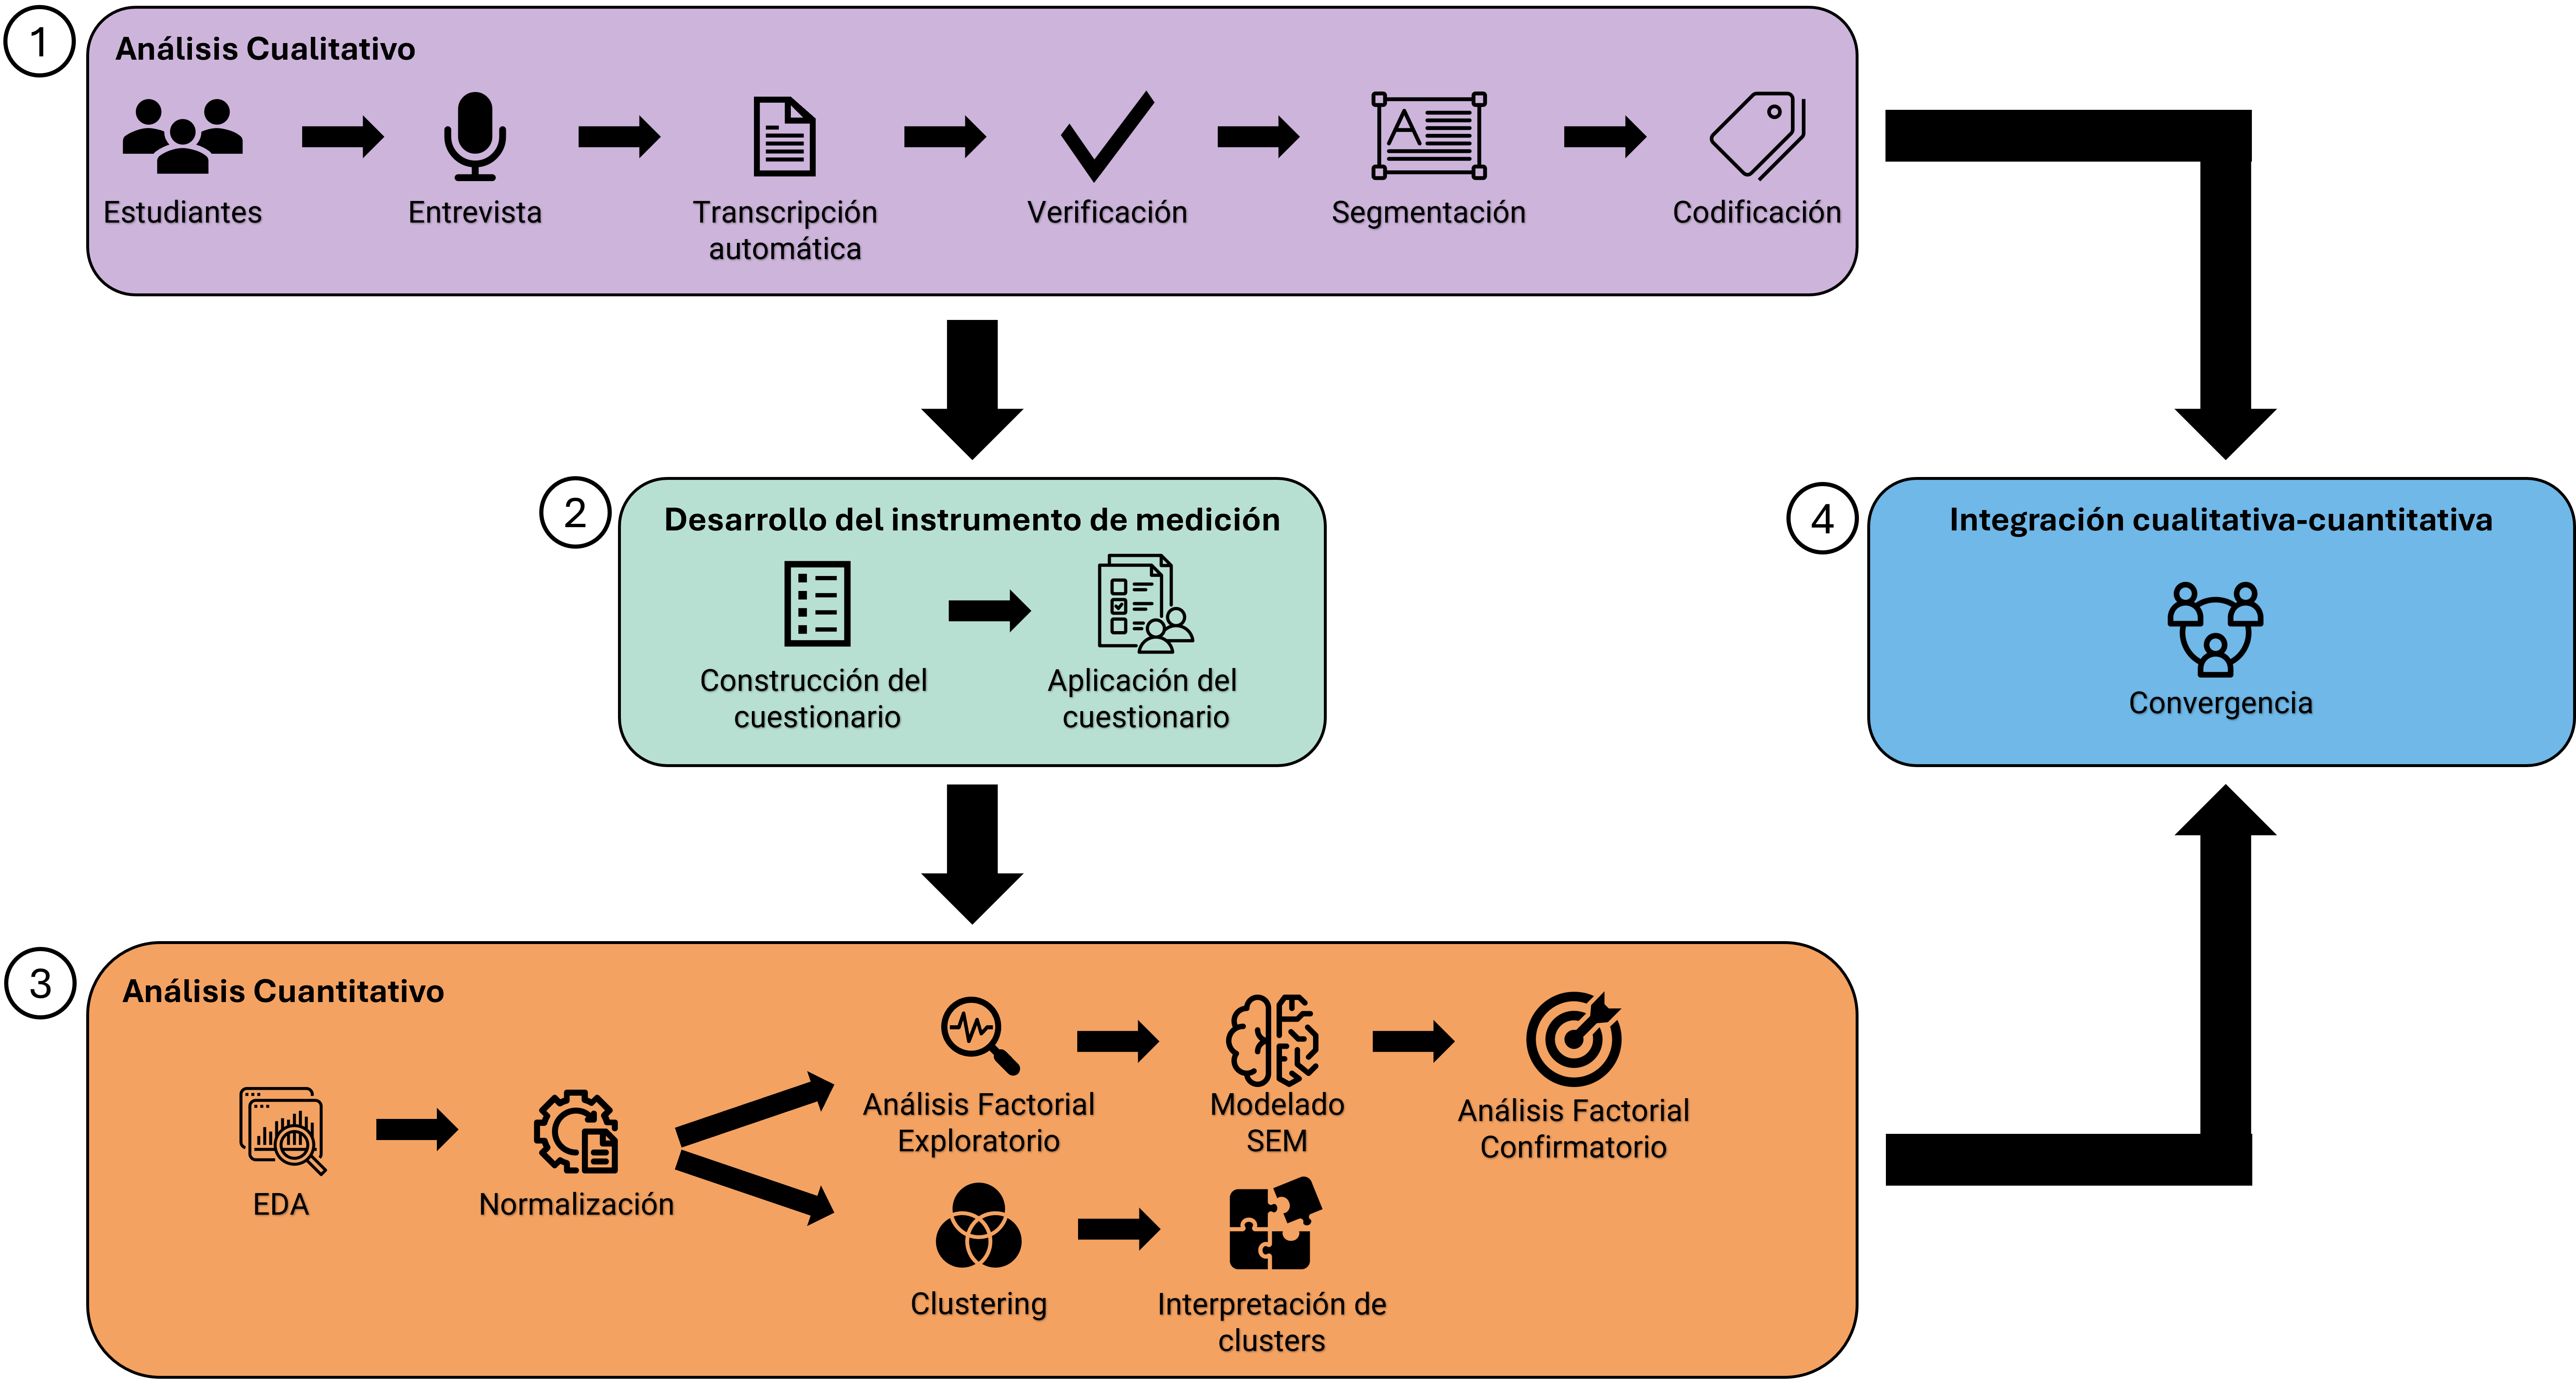
\includegraphics[width=0.8\textwidth]{img/metodo_mixto_4_fases.png}
    \caption{Flujo del proceso de aplicación del diseño secuencial exploratorio.}
    \label{fig:metodo_mixto}
\end{figure*}

\subsection{Análisis cualitativo}

La fase cualitativa tuvo como objetivo explorar la experiencia de los estudiantes universitarios que recibieron clases virtuales durante la pandemia de COVID-19 y que posteriormente retornaron a la presencialidad. Para ello, se realizaron entrevistas a una muestra de estudiantes de la Universidad de Cuenca. El diseño de las entrevistas buscó capturar dimensiones pedagógicas, tecnológicas, emocionales y sociales de la experiencia educativa virtual.

Las entrevistas fueron grabadas en audio y sometidas a un proceso de transcripción automática, la cual fue posteriormente revisada de forma manual para garantizar la fidelidad del texto. A partir de las transcripciones revisadas, se identificaron segmentos textuales relevantes que fueron codificados. Cada código encontrado representaba una idea o concepto de lo que expresaban los estudiantes.

Posteriormente, se refinaron algunos de estos códigos mediante la derivación de subcódigos que capturaban matices específicos dentro de una categoría más amplia. Finalmente, se agruparon códigos afines en temas cualitativos que representan dimensiones interpretativas de orden superior.

Como resultado de este proceso, se identificaron 26 códigos únicos, los cuales fueron organizados en seis temas cualitativos. La tabla \ref{tab:temas_codigos} presenta la estructura completa del marco cualitativo.

\begin{table*}[!htb]
\centering
\footnotesize
\begin{tabular}{p{0.8cm}p{5.2cm}p{7cm}}
\toprule
\textbf{N\textordmasculine} & \textbf{Tema} & \textbf{Códigos} \\
\midrule
T1 & Limitaciones del aprendizaje on-line & Desafíos de aprendizaje, Desafíos tecnológicos, Participación, Asignaturas, Experiencia colectiva, Resultados académicos, Desventajas edu.\ on-line \\
T2 & Distracción (Sobreposición de educación, casa y entretenimiento) & Atención, Ambigüedad del espacio, Cámara, Cansancio, Emociones \\
T3 & ¿Vigilar y no sancionar? (Flexibilización de normas académicas) & Evaluación, Copia, Resultados académicos, Cámara \\
T4 & El docente on-line (la difícil transición de profesor a facilitador) & Estrategias de enseñanza, Aprendizajes, Traducción digital, Intraductibilidad, Rol del docente, Comunicación, Relación docente-estudiante \\
T5 & ``Un retorno feliz'' (la educación cara a cara) & Presencialidad, Participación, Atención, Evaluación, Resultados académicos \\
T6 & Empleo de la tecnología en postpandemia & Competencias adquiridas, Ventajas edu.\ on-line, Clases postpandemia, Aprendizaje y uso de IA \\
\bottomrule
\end{tabular}
\caption{Temas cualitativos y códigos asociados.}
\label{tab:temas_codigos}
\end{table*}

Este marco cualitativo constituyó la base conceptual sobre la cual se construyó el instrumento de medición, garantizando que las variables medidas estuvieran arraigadas en las experiencias reales de los estudiantes.

\subsection{Desarrollo del instrumento de medición}

El cuestionario se diseñó como puente entre las fases cualitativa y cuantitativa. Cada pregunta se vinculó manualmente con uno o varios códigos o subcódigos del marco cualitativo, asegurando así la trazabilidad entre los hallazgos de las entrevistas y las variables cuantitativas.

El instrumento resultante constó de 38 preguntas, de las cuales 33 fueron utilizadas para el análisis cuantitativo, debido a que las primeras cinco preguntas correspondían a variables demográficas. Las preguntas adoptaron diversos formatos de respuesta como ítems dicotómicos, escalas Likert de 4 puntos y preguntas de opción múltiple con única respuesta. La tabla \ref{tab:mapeo_preguntas} ilustra un ejemplo de la relación entre preguntas seleccionadas, códigos y subcódigos del marco cualitativo.

\begin{table*}[!htb]
\centering
\footnotesize
\begin{tabular}{p{1cm}p{5.5cm}p{3.3cm}p{3.2cm}}
\toprule
\textbf{Preg.} & \textbf{Enunciado} & \textbf{Códigos} & \textbf{Subcódigos} \\
\midrule
6 & De la siguiente lista, ¿cuáles fueron las dificultades de aprendizaje que usted enfrentó durante las clases virtuales? & Desafíos de aprendizaje, Desafíos tecnológicos, Emociones, Estrategias de enseñanza, Desventajas edu.\ on-line & Participación, Atención, Acceso, Destrezas digitales, Traducción digital \\
11 & ¿Cuáles de los siguientes distractores experimentó durante las clases virtuales? & Atención, Ambigüedad del espacio, Cansancio \\
12 & Durante las clases virtuales, ¿usted experimentó alguna de las siguientes emociones? & Emociones & --- \\
16 & ¿Qué factores usted asocia al cansancio durante las clases virtuales?
 & Estrategias de enseñanza & Pantalla, Cansancio, Traducción digital, Ambigüedad del espacio \\
25 & Estrategias de enseñanza que más aportaron & Estrategias de enseñanza, Aprendizaje & Traducción digital, Aprendizaje práctico, Experiencia colectiva \\
\bottomrule
\end{tabular}
\caption{Ejemplos de correspondencia entre preguntas del cuestionario y códigos/subcódigos cualitativos.}
\label{tab:mapeo_preguntas}
\end{table*}

Este proceso de mapeo sistemático permitió preservar la correspondencia conceptual entre los hallazgos cualitativos y su posterior evaluación cuantitativa. En consecuencia, el cuestionario no se limitó a medir constructos definidos de manera abstracta, sino que incorporó las dimensiones específicas identificadas a partir del discurso de los estudiantes, proporcionando una base empírica para su posterior análisis y validación estructural.

Finalmente, el cuestionario fue aplicado a 513 estudiantes universitarios pertenecientes a las distintas facultades de la Universidad de Cuenca. Estos datos constituyen la base para el desarrollo de los análisis cuantitativos posteriores.

\subsection{Análisis cuantitativo}

A partir de los datos recolectados tras la aplicación del cuestionario se desarrollaron varios bloques analíticos interdependientes, correspondientes al análisis exploratorio de datos, al clustering, al análisis factorial exploratorio y al análisis factorial confirmatorio. En los apartados siguientes se describe cada uno de estos componentes junto con sus resultados y discusión inmediata.

\subsubsection{Análisis exploratorio de datos (EDA)}

El EDA constituyó la primera etapa del análisis cuantitativo, orientada a caracterizar la estructura general del conjunto de datos antes de aplicar técnicas multivariadas más complejas. Este análisis se organizó en dos niveles complementarios. En el análisis univariado se calcularon estadísticos descriptivos como la media, mediana, desviación estándar, valores mínimo y máximo, rango y cuartiles para variables numéricas, así como distribuciones de frecuencia absolutas y relativas y moda para variables categóricas.

En el análisis bivariado se evaluó la asociación estadística entre pares de variables categóricas mediante la prueba de chi-cuadrado ($\chi^2$), complementada con la corrección de Benjamini-Hochberg \cite{FDR} para el control de la tasa de falsos descubrimientos (FDR, $q \leq 0.05$). Siguiendo las recomendaciones propuestas en \cite{cohen1988statistical}, la magnitud de las asociaciones se cuantificó mediante el coeficiente $\phi$ en tablas $2 \times 2$ y con $V$ de Cramér en tablas de mayor dimensionalidad. Se adoptó un umbral de relevancia práctica de $0.20$ para ambos coeficientes, al considerarse un valor intermedio entre un tamaño de efecto pequeño y uno mediano \cite{cohen1988statistical}.

Posteriormente, los datos fueron sometidos a un proceso de normalización y codificación previo a la aplicación de técnicas de clustering y análisis factoriales. Las variables categóricas fueron transformadas mediante codificación one-hot \cite{wold_model_1957} para los ítems de respuesta múltiple y codificación ordinal para las escalas Likert. A partir de este preprocesamiento se estructuraron dos versiones del conjunto de datos: una versión desagregada, que conservó la alta dimensionalidad del instrumento al tratar cada subítem como una variable independiente; y una versión agrupada, que redujo dicha dimensionalidad mediante la suma de los subítems de cada pregunta, consolidándolos en un único indicador por pregunta.

En consecuencia, se detectó que la muestra con los datos desagregados estuvo conformada por estudiantes con una edad media de 22.70 años (con un rango entre 19 y 34 años) y un claro predominio femenino (61.21\%). Las características descriptivas más relevantes se presentan en la tabla~\ref{tab:univariado}.

Los datos revelan que las clases virtuales estuvieron marcadas por una alta incidencia de distractores y problemas técnicos, lo que explica que más de la mitad de los participantes (56.34\%) percibiera un aprendizaje menor durante la pandemia. A ello se suma un panorama emocional dominado por el estrés, la monotonía y el aislamiento, con depresión y soledad afectando a cerca de la mitad de los estudiantes.

No obstante, la presencia de emociones positivas como la gratitud, confianza y proactividad en aproximadamente un tercio de la muestra indica que, incluso en un contexto adverso, un subgrupo logró afrontar las dificultades de las emociones negativas y adaptarse positivamente al nuevo entorno virtual. En cuanto al uso de inteligencia artificial, su aceptación fue casi universal (91\% de acuerdo) y ChatGPT se posicionó como la herramienta más utilizada con una media de $2.89$ en escala de Likert de 4 puntos y una desviación estándar de $0.95$. Entre las actividades para las cuales más se utiliza la IA destacan la búsqueda de información y la generación de ideas. Esta elevada adopción, valorada como ética por el 84\%, refleja una integración acelerada de la IA en las prácticas académicas.

\begin{table}[htbp]
\centering
%\begin{tabular}{@{}p{0.70\textwidth}c@{}}
\setlength{\tabcolsep}{1pt}
\begin{tabular}{@{}p{0.75\columnwidth}c@{}}
\toprule
\multicolumn{2}{@{}l}{\textbf{Sociodemografía y percepción del aprendizaje}} \\
\midrule
Edad (años), $M$ (rango) & 22.70 (19--34) \\
Género femenino & 61.21\% \\
\addlinespace
\multicolumn{2}{@{}l}{\textit{Facultades con mayor representación}} \\
\quad Ciencias Médicas & 15.40\% \\
\quad Ciencias Económicas y Administrativas & 14.62\% \\
\quad Ingeniería & 12.28\% \\
Número de facultades & 12 \\
Número de carreras & 23 \\
\addlinespace
\multicolumn{2}{@{}l}{\textit{Percepción del aprendizaje durante la pandemia}} \\
\quad Menor & 56.34\% \\
\quad Igual & 28.07\% \\
\quad Mayor & 15.59\% \\
Preferencia por modalidad presencial & 88.70\% \\
Presencialidad valorada importante/muy importante & 87.72\% \\
Profesores jóvenes se adaptaron más fácilmente & 72.32\% \\
\midrule
\multicolumn{2}{@{}l}{\textbf{Dificultades y distractores}} \\
\midrule
\multicolumn{2}{@{}l}{\textit{Dificultades de aprendizaje}} \\
\quad Elementos distractores & 88\% \\
\quad Problemas técnicos & 82\% \\
\quad Metodología de enseñanza & 82\% \\
\addlinespace
\multicolumn{2}{@{}l}{\textit{Distractores específicos}} \\
\quad Entretenimiento en dispositivos & 90\% \\
\quad Interrupción de la conexión a internet & 89\% \\
\quad Cansancio & 77\% \\
\midrule
\multicolumn{2}{@{}l}{\textbf{Emociones}} \\
\midrule
\multicolumn{2}{@{}l}{\textit{Negativas}} \\
\quad Estrés & 82\% \\
\quad Monotonía & 81\% \\
\quad Aislamiento & 76\% \\
\quad Ansiedad & 71\% \\
\quad Soledad & 54\% \\
\quad Depresión & 51\% \\
\addlinespace
\multicolumn{2}{@{}l}{\textit{Positivas}} \\
\quad Gratitud & 39\% \\
\quad Confianza & 36\% \\
\quad Proactividad & 32\% \\
\midrule
\multicolumn{2}{@{}l}{\textbf{Uso de inteligencia artificial}} \\
\midrule
Acuerdo con el uso de IA en la formación & 91\% \\
Consideración ética del uso de IA & 84\% \\
ChatGPT, $M$ ($DE$) [escala 1--4] & 2.89 (0.95) \\
\addlinespace
\multicolumn{2}{@{}l}{\textit{Actividades más frecuentes}} \\
\quad Búsqueda de información & 86\% \\
\quad Generación de ideas & 81\% \\
\quad Estructuración de textos & 63\% \\
\bottomrule
\end{tabular}
\caption{Estadísticos descriptivos del análisis univariado.}
\label{tab:univariado}
\end{table}

A partir del análisis bivariado aplicado se identificaron 318 asociaciones significativas, de las cuales 124 mostraron tamaños del efecto moderados o altos ($\phi \geq 0.25$ o $V \geq 0.20$). Las ocho asociaciones de mayor magnitud ($\phi \geq 0.39$) se ilustran en la tabla~\ref{tab:bivariado}, donde todas ellas reportan un $p < 0.001$.

\begin{table}[htbp]
\centering
\begin{tabular}{@{}p{0.90\columnwidth}c@{}}
\toprule
\textbf{Asociación} & \textbf{$\phi$} \\
\midrule
Problemas técnicos --- Interrupción de internet & 0.53 \\
Depresión --- Malestar psicológico & 0.51 \\
Depresión --- Soledad & 0.48 \\
Estrés --- Presión & 0.46 \\
Problemas técnicos --- Apagado de cámara (conectividad) & 0.44 \\
Intercambio de información (redes sociales) --- Actividad grupal & 0.42 \\
Gratitud --- Confianza & 0.40 \\
Gratitud --- Proactividad & 0.39 \\
\bottomrule
\end{tabular}
\caption{Asociaciones bivariadas con mayor tamaño de efecto ($\phi \geq 0.39$).}
\label{tab:bivariado}
\end{table}

La asociación más robusta se observó entre problemas técnicos como dificultad de aprendizaje e interrupción de internet, donde el 96.92\% de quienes reportaron problemas técnicos también experimentaron interrupciones de internet, efecto que se extendió al apagado de cámara por conectividad. En el dominio emocional, depresión, malestar psicológico, soledad y estrés conforman una densa red de malestar interconectado. Estos patrones evidencian que las barreras tecnológicas no solo dificultan el aprendizaje, sino que amplifican la desconexión y pueden influir en el malestar psicológico.  

De forma complementaria, las emociones positivas mostraron un agrupamiento diferenciado. La gratitud se asoció con confianza y proactividad, revelando un perfil de afrontamiento positivo que opera de manera independiente del polo negativo. Esto sugiere que no todos los estudiantes reaccionaron de forma homogénea debido a que alrededor de un tercio logró afrontar las dificultades emocionales. En cuanto a la deshonestidad académica, el intercambio de información por redes sociales se vinculó con la actividad grupal y con la búsqueda de información en internet durante exámenes, lo que apunta a prácticas colaborativas no autorizadas facilitadas por el entorno virtual.

Estas asociaciones bivariadas ofrecen un primer nivel de corroboración con los hallazgos cualitativos. Confirman que las relaciones observadas en el discurso —como la conexión entre problemas técnicos y distractores, o entre emociones negativas y malestar— se mantienen al ser examinadas estadísticamente en una muestra amplia. Los tamaños del efecto, que superan ampliamente los umbrales convencionales para efectos grandes, dotan de solidez inferencial a estos vínculos y sientan las bases para los análisis multivariados posteriores, orientados a modelar trayectorias de riesgo y protección en la experiencia educativa virtual.

\subsubsection{Normalización}
Con el fin de preparar los datos para el análisis factorial exploratorio y el de clustering, se realizó una etapa de preprocesamiento orientada a homogeneizar la escala de las variables numéricas. Para ello, se aplicó una estandarización mediante puntuaciones \textit{z-score} \cite{illowsky2013introductory}, transformando los valores de modo que presentaran una media de cero y una desviación estándar de uno. Esta transformación permitió reducir la influencia de las diferencias de escala entre las variables y evitar que aquellas con mayores magnitudes dominaran los análisis posteriores, particularmente el análisis de clustering, donde las distancias entre observaciones desempeñan un papel fundamental.

\subsubsection{Aplicación de clustering e interpretación de grupos}

El clustering tuvo como objetivo identificar perfiles diferenciados de estudiantes a partir de patrones multivariados en sus respuestas, utilizando el conjunto de datos desagregado para preservar su variabilidad intrínseca. Para abordar la alta dimensionalidad del espacio original, se evaluaron experimentalmente tres técnicas de reducción dimensional: PCA \cite{noauthor_analysis_nodate}, t-SNE \cite{maaten_visualizing_2008} y UMAP \cite{mcinnes_umap_2020}, como alternativas independientes de transformación previa al clustering. Estas técnicas se combinaron con seis algoritmos de clustering: K-Means \cite{macqueen_methods_1967}, Agglomerative Clustering \cite{noauthor_hierarchical_nodate}, DBSCAN \cite{ester_density-based_1996}, BIRCH \cite{zhang_birch_1996}, Gaussian Mixture Models (GMM) \cite{noauthor_maximum_nodate} y OPTICS \cite{ankerst_optics_1999}, evaluando distintas configuraciones para analizar su desempeño.

Para cada combinación de técnica de reducción de dimensionalidad y algoritmo de clustering, se realizó una búsqueda aleatoria (\textit{Random Search}) sobre el espacio de hiperparámetros. Cada partición obtenida fue evaluada mediante tres métricas complementarias de validación: el coeficiente de Silhouette \cite{rousseeuw_silhouettes_1987}, el índice de Davies-Bouldin \cite{noauthor_cluster_nodate} y el índice de Calinski-Harabasz \cite{calinski_dendrite_1974}. El mejor experimento se seleccionó mediante un criterio de balance entre las tres métricas, incorporando además una penalización para particiones con clústeres excesivamente desbalanceados, donde uno de los grupos concentra casi la totalidad de las observaciones y los demás presentan tamaños marginales, lo que limita su utilidad para la caracterización de perfiles estudiantiles diferenciados.

Después de haber identificado el experimento óptimo, se realizó la caracterización de los clústeres con el apoyo de modelos de lenguaje de gran escala (LLM). Para ello, se proporcionaron estadísticas descriptivas como medias y medianas, junto a los resultados de las pruebas $\chi^2$ con corrección FDR aplicadas dentro de cada grupo encontrado. Esta información permitió generar una interpretación de los clústeres basada en sus principales características diferenciadoras.

Mediante el análisis de clustering se identificó una partición óptima utilizando el algoritmo K-Means en conjunto con la reducción de dimensionalidad UMAP y un $k=6$. La tabla~\ref{tab:clusters} presenta los seis perfiles diferenciados, su descripción y el porcentaje de instancias que agrupan. Esta tipología muestra que la respuesta a la virtualidad no fue homogénea debido a que se encontraron varios perfiles que van desde estudiantes que, pese a las dificultades técnicas, compensan con emociones positivas (\textit{Tecnófilos resilientes}), hasta aquellos que concentran el máximo malestar en aspectos tecnológicos y emocionales (\textit{Críticamente afectados}). La emergencia de un perfil con alta monotonía pero elevada gratitud (\textit{Monótonos pero agradecidos}) refuerza la bidimensionalidad emocional identificada previamente, mientras que el conglomerado \textit{Sobrecargados por cuidados} evidencia el peso de las responsabilidades domésticas como factor diferenciador.

\begin{table}[htbp]
\centering
\begin{tabular}{@{}c p{0.68\columnwidth} r@{}}
\toprule
\textbf{Clúster} & \textbf{Descripción} & \textbf{\% datos} \\
\midrule
1 & \textit{Tecnófilos resilientes}: altos problemas técnicos, elevada gratitud, proactividad y confianza. & 12.8\% \\
2 & \textit{Sobrecargados por cuidados}: alta carga de cuidado de dependientes y actividades domésticas, baja adopción de IA. & 16.4\% \\
3 & \textit{Estresados digitales}: máximas emociones negativas (estrés 95.8\%, ansiedad 87.5\%) y uso intensivo de IA. & 18.7\% \\
4 & \textit{Adaptados exitosos}: menores dificultades técnicas, mínima presencia de emociones negativas, alta motivación, preferencia presencial. & 18.5\% \\
5 & \textit{Monótonos pero agradecidos}: elevada monotonía (96.5\%), alta gratitud y confianza (confirma bidimensionalidad emocional). & 16.6\% \\
6 & \textit{Críticamente afectados}: máximas dificultades técnicas y emociones negativas en todos los dominios evaluados. & 17.0\% \\
\bottomrule
\end{tabular}
\caption{Perfiles de estudiantes obtenidos mediante clustering.}
\label{tab:clusters}
\end{table}

La identificación de estos seis perfiles no solo confirma la heterogeneidad de la experiencia estudiantil, sino que proporciona una tipología empírica que puede orientar intervenciones diferenciadas. Por ejemplo, los \textit{Tecnófilos resilientes} podrían beneficiarse de estrategias que potencien su actitud positiva frente a la tecnología, mientras que los \textit{Críticamente afectados} requerirían apoyo psicosocial y técnico intensivo. La existencia de un perfil \textit{Monótonos pero agradecidos} es particularmente relevante porque demuestra que la monotonía, a pesar de ser una emoción negativa, no necesariamente anula la gratitud, lo que sugiere que las intervenciones podrían enfocarse en cultivar emociones positivas incluso en contextos de alta monotonía.

\subsubsection{Exploración y validación del modelo de ecuaciones estructurales}

Esta sección comprende los distintos análisis realizados para la exploración, evaluación y validación de la estructura factorial y del modelo de ecuaciones estructurales, mediante el análisis factorial exploratorio, el modelado de ecuaciones estructurales y el análisis factorial confirmatorio.

\vspace{0.5em}
\noindent\textbf{Análisis Factorial Exploratorio}

El AFE se ejecutó de manera independiente sobre ambas versiones del conjunto de datos: la desagregada (112 subítems individuales) y la agrupada (33 preguntas consolidadas). Con el fin de asegurar la factorizabilidad de los datos, el procedimiento incorporó un filtrado iterativo paso a paso basado en el índice de Kaiser-Meyer-Olkin (KMO). En cada iteración, se calculó la medida de adecuación muestral individual (\textit{Measure of Sampling Adequacy}, MSA) de cada variable, eliminando progresivamente aquella con el menor valor cuando este no alcanzaba el umbral de $0.70$ y recalculando la matriz de correlaciones, hasta que todas las variables retenidas y el KMO global superaran dicho valor crítico, de acuerdo con la recomendación de \cite{kaiser1974index}.

Posteriormente, se aplicó la prueba de esfericidad de Bartlett para evaluar la adecuación de la matriz de correlaciones, considerando evidencia estadística de correlación entre variables cuando $p < 0.05$. Finalmente, se realizó un análisis de componentes principales (PCA) con rotación ortogonal Varimax, reteniendo los componentes necesarios para explicar al menos el 80\% de la varianza acumulada, con el propósito de obtener una representación reducida que favoreciera la interpretación de los factores extraídos.

La tabla~\ref{tab:efa_resumen} resume los resultados para ambas versiones de los datos. En ambos casos, la prueba de esfericidad de Bartlett fue significativa ($p < 0.001$) y el KMO global superó el umbral de 0.70, confirmando la adecuación de los datos para el análisis factorial.

\begin{table}[!htb]
\centering
\footnotesize
\begin{tabular}{lcc}
\toprule
\textbf{Métrica} & \textbf{Desagregado} & \textbf{Agrupado} \\
\midrule
Variables iniciales & 112 & 33 \\
Variables retenidas (KMO) & 61 & 16 \\
KMO global & 0.82 & 0.79 \\
Bartlett $\chi^2$ & 8035.89 & 1139.28 \\
Bartlett $p$ & $<0.001$ & $<0.001$ \\
Componentes (80\% var.) & 35 & 11 \\
Varianza acumulada & 80.85\% & 83.22\% \\
\bottomrule
\end{tabular}
\caption{Resumen del Análisis Factorial Exploratorio.}
\label{tab:efa_resumen}
\end{table}

El AFE sobre el conjunto desagregado requirió la retención de 61 variables (de 112 iniciales) para alcanzar un KMO adecuado, mientras que en el conjunto agrupado se retuvieron 16 variables. La varianza explicada fue ligeramente superior en el conjunto agrupado (83.22\%) con solo 11 componentes, frente a los 35 componentes del conjunto desagregado. Esta diferencia refleja la mayor complejidad y granularidad del conjunto desagregado, que preserva toda la variabilidad de los subítems.

La matriz rotada Varimax obtenida del AFE (no mostrada en su totalidad por razones de espacio) reveló agrupaciones coherentes de variables que correspondían a dimensiones como emociones negativas, emociones positivas, problemas técnicos, distractores, uso de IA y preferencia por la presencialidad. Estas agrupaciones sirvieron como insumo fundamental para la especificación de los modelos SEM, tanto los generados por inteligencia artificial como los construidos manualmente.

\vspace{0.5em}
\noindent\textbf{Modelado SEM}

Los resultados del AFE, incluyendo la matriz de cargas factoriales rotada mediante Varimax y la varianza explicada por cada componente, fueron utilizados como insumo para dos modelos de lenguaje de gran escala (LLM): Gemini y DeepSeek. La incorporación de estos modelos tuvo como propósito apoyar la especificación tanto del modelo de medición como del modelo estructural del SEM, aprovechando su capacidad para consultar y sintetizar literatura científica relevante y reciente. En particular, los modelos fueron utilizados como herramientas de apoyo para identificar posibles relaciones entre los constructos y fundamentar su representación dentro del modelo propuesto. Las referencias y relaciones sugeridas por los modelos fueron posteriormente verificadas, contrastándolas con la literatura científica original, con el fin de asegurar la pertinencia y validez de las decisiones adoptadas en la especificación del modelo.

A partir de los resultados de la etapa anterior, los modelos fueron instruidos para inferir variables latentes mediante las agrupaciones identificadas en la matriz rotada y formular modelos SEM que incorporaran tanto el modelo de medición como el modelo estructural. Las relaciones propuestas entre variables latentes fueron fundamentadas en la literatura sobre educación virtual. Cada modelo de inteligencia artificial generó dos propuestas de SEM, una para el conjunto de datos desagregado y otra para el conjunto agrupado.

Adicionalmente, se evaluaron tres modelos SEM complementarios. El primero correspondió al modelo de medición original definido durante la estructuración de la encuesta, acompañado de un modelo estructural fundamentado en la revisión de la literatura sobre el estado del arte. Los modelos segundo y tercero se desarrollaron a partir de modificaciones del modelo inicial y de un proceso iterativo de experimentación, con el objetivo de explorar configuraciones alternativas en las relaciones entre variables latentes.

En total, se evaluaron diez modelos SEM correspondientes a las distintas configuraciones de los conjuntos de datos agrupado y desagregado. Estos modelos incluyeron las especificaciones propuestas por Gemini y DeepSeek, además del modelo original y sus dos variantes derivadas. Para cada modelo se calcularon tres indicadores de fiabilidad por constructo: el alfa de Cronbach \cite{Cronbach1951}, el omega de McDonald \cite{mcdonald1999test} y la fiabilidad compuesta (CR) \cite{FornellLarcker1981}. Como criterios principales de evaluación se priorizaron el omega de McDonald y la CR, debido a que el omega resulta adecuado cuando existen diferencias en las cargas factoriales de las variables observadas \cite{mcdonald1999test}, mientras que la fiabilidad compuesta constituye una medida recomendada para evaluar la fiabilidad en modelos SEM \cite{raykov1997estimation}.

El modelo construido con el apoyo de DeepSeek y utilizando los datos agrupados se ilustra en la tabla~\ref{tab:sem_modelo}. La estructura obtenida muestra variables latentes consistentes con los hallazgos de los análisis previos. Por ejemplo, la variable latente \textit{Experiencia de aprendizaje virtual} agrupa indicadores relacionados con las emociones durante las clases virtuales, las dificultades de aprendizaje y las razones para apagar la cámara, en concordancia con el clúster 6 (\textit{Críticamente afectados}) identificado en el análisis de clustering y con la asociación entre dificultades de aprendizaje, problemas técnicos y apagado de cámara observada en el análisis bivariado (tabla~\ref{tab:bivariado}). Asimismo, el modelo incorpora variables latentes vinculadas con la preferencia por la modalidad presencial, resultado que coincide con el análisis univariado (tabla~\ref{tab:univariado}), donde se evidencia que la mayoría de los estudiantes prefiere las clases presenciales.

\begin{table}[htbp]
\centering
\begin{tabular}{>{\raggedright\arraybackslash}p{0.28\linewidth} 
                >{\raggedright\arraybackslash}p{0.60\linewidth}}
\toprule
\multicolumn{2}{c}{\textbf{Modelo de medición (formativo)}} \\
\midrule
Experiencia aprendizaje virtual 
    & $\leftarrow$ Emociones durante clases virtuales; Dificultades de aprendizaje; Razones para apagar la cámara. \\
Presencialidad digital
    & $\leftarrow$ Recursos digitales posteriores; Motivación hacia la modalidad presencial. \\
Preferencia presencialidad 
    & $\leftarrow$ Preferencia de modalidad; Importancia de la presencialidad. \\
Cansancio por distractores virtuales 
    & $\leftarrow$ Razones de cansancio; Distractores durante las clases virtuales. \\
\midrule
\multicolumn{2}{c}{\textbf{Modelo estructural}} \\
\midrule
Motivación virtuales 
    & $\begin{aligned}[t]
      = &\text{Experiencia aprendizaje virtual} \\
      &+ \text{Presencialidad digital} \\
      &+ \text{Preferencia presencialidad} \\
      &+ \text{Cansancio por distractores virtuales}
      \end{aligned}$ \\
\midrule
\multicolumn{2}{c}{\textbf{Correlaciones entre variables latentes}} \\
\midrule
Experiencia aprendizaje virtual 
    & $\leftrightarrow$ Presencialidad digital; Preferencia presencialidad; Cansancio por distractores virtuales. \\
Presencialidad digital 
    & $\leftrightarrow$ Preferencia presencialidad; Cansancio por distractores virtuales. \\
Preferencia presencialidad 
    & $\leftrightarrow$ Cansancio por distractores virtuales. \\
\bottomrule
\end{tabular}

\medskip
\small{\textit{Nota:} $\leftarrow$ indica la formación de la variable latente a partir de las variables observadas;
$\leftrightarrow$ indica covarianza entre latentes.}
\caption{Especificación SEM propuesta con DeepSeek utilizando datos agrupados.}
\label{tab:sem_modelo}
\end{table}

Por otra parte, en la figura~\ref{fig:sem_deepseek_desagregado} se presenta el modelo de medición construido a partir de los datos desagregados. Aunque este modelo no alcanza índices de ajuste elevados, logra capturar relaciones consistentes con los resultados obtenidos en los análisis previos y aporta evidencia para desagregar algunos de los códigos planteados inicialmente en el análisis cualitativo. En conjunto, estos resultados, junto con los clústeres identificados, permiten validar y contrastar los temas cualitativos inicialmente planteados, tal y como se muestra en la figura~\ref{fig:relacion_cuali_cuanti}.

\begin{figure*}[!htb]
  \centering
  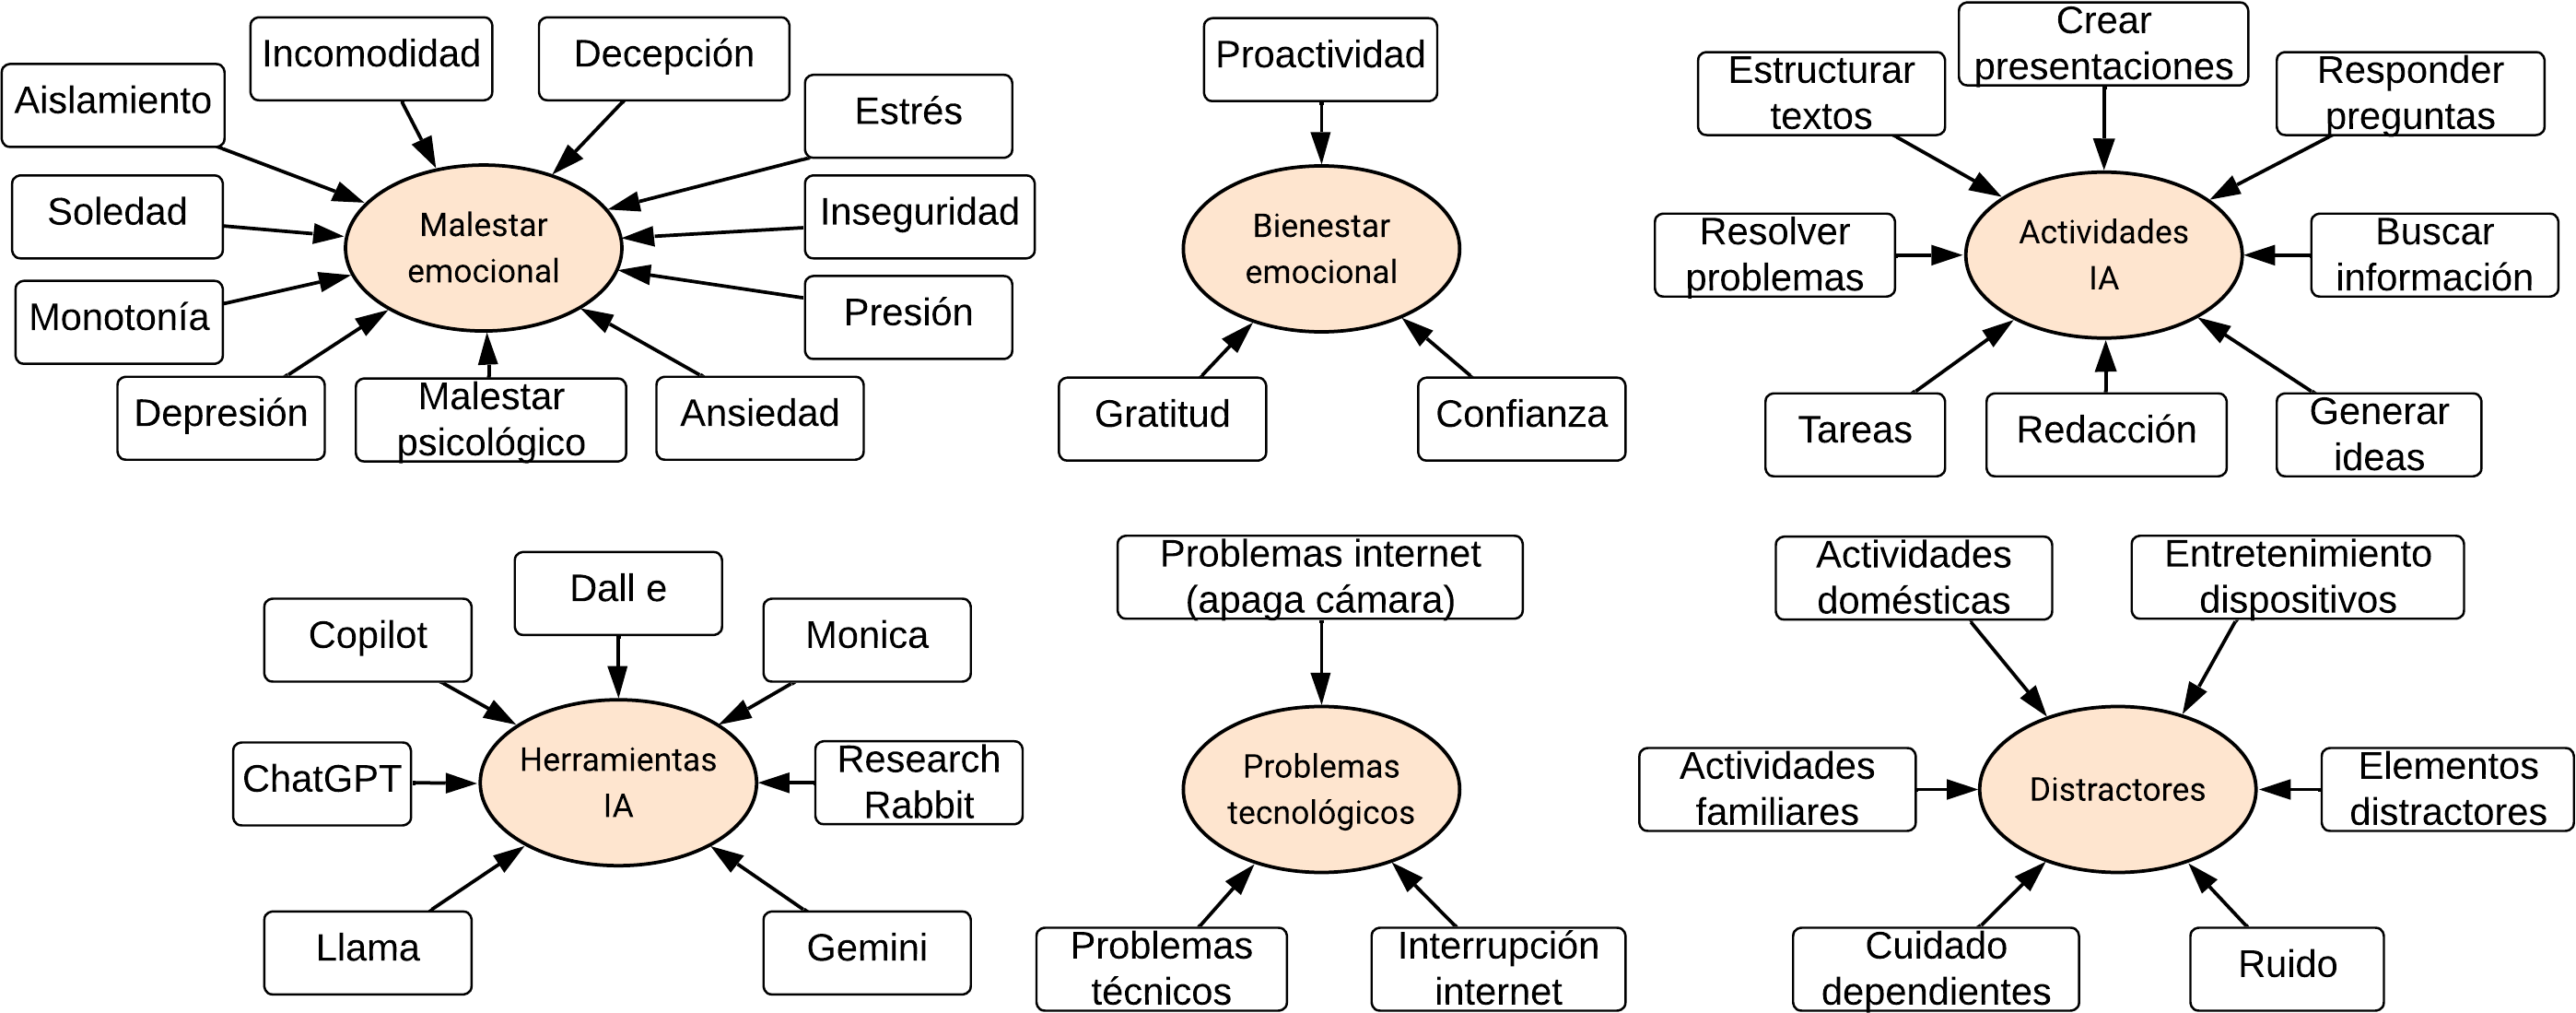
\includegraphics[width=0.8\textwidth]{img/sem/sem_deepseek_medicion.png}
  \caption{Modelo de medición del SEM creado utilizando DeepSeek y el conjunto de datos desagregado.}
  \label{fig:sem_deepseek_desagregado}
\end{figure*}

\begin{figure}[!htb]
    \centering
    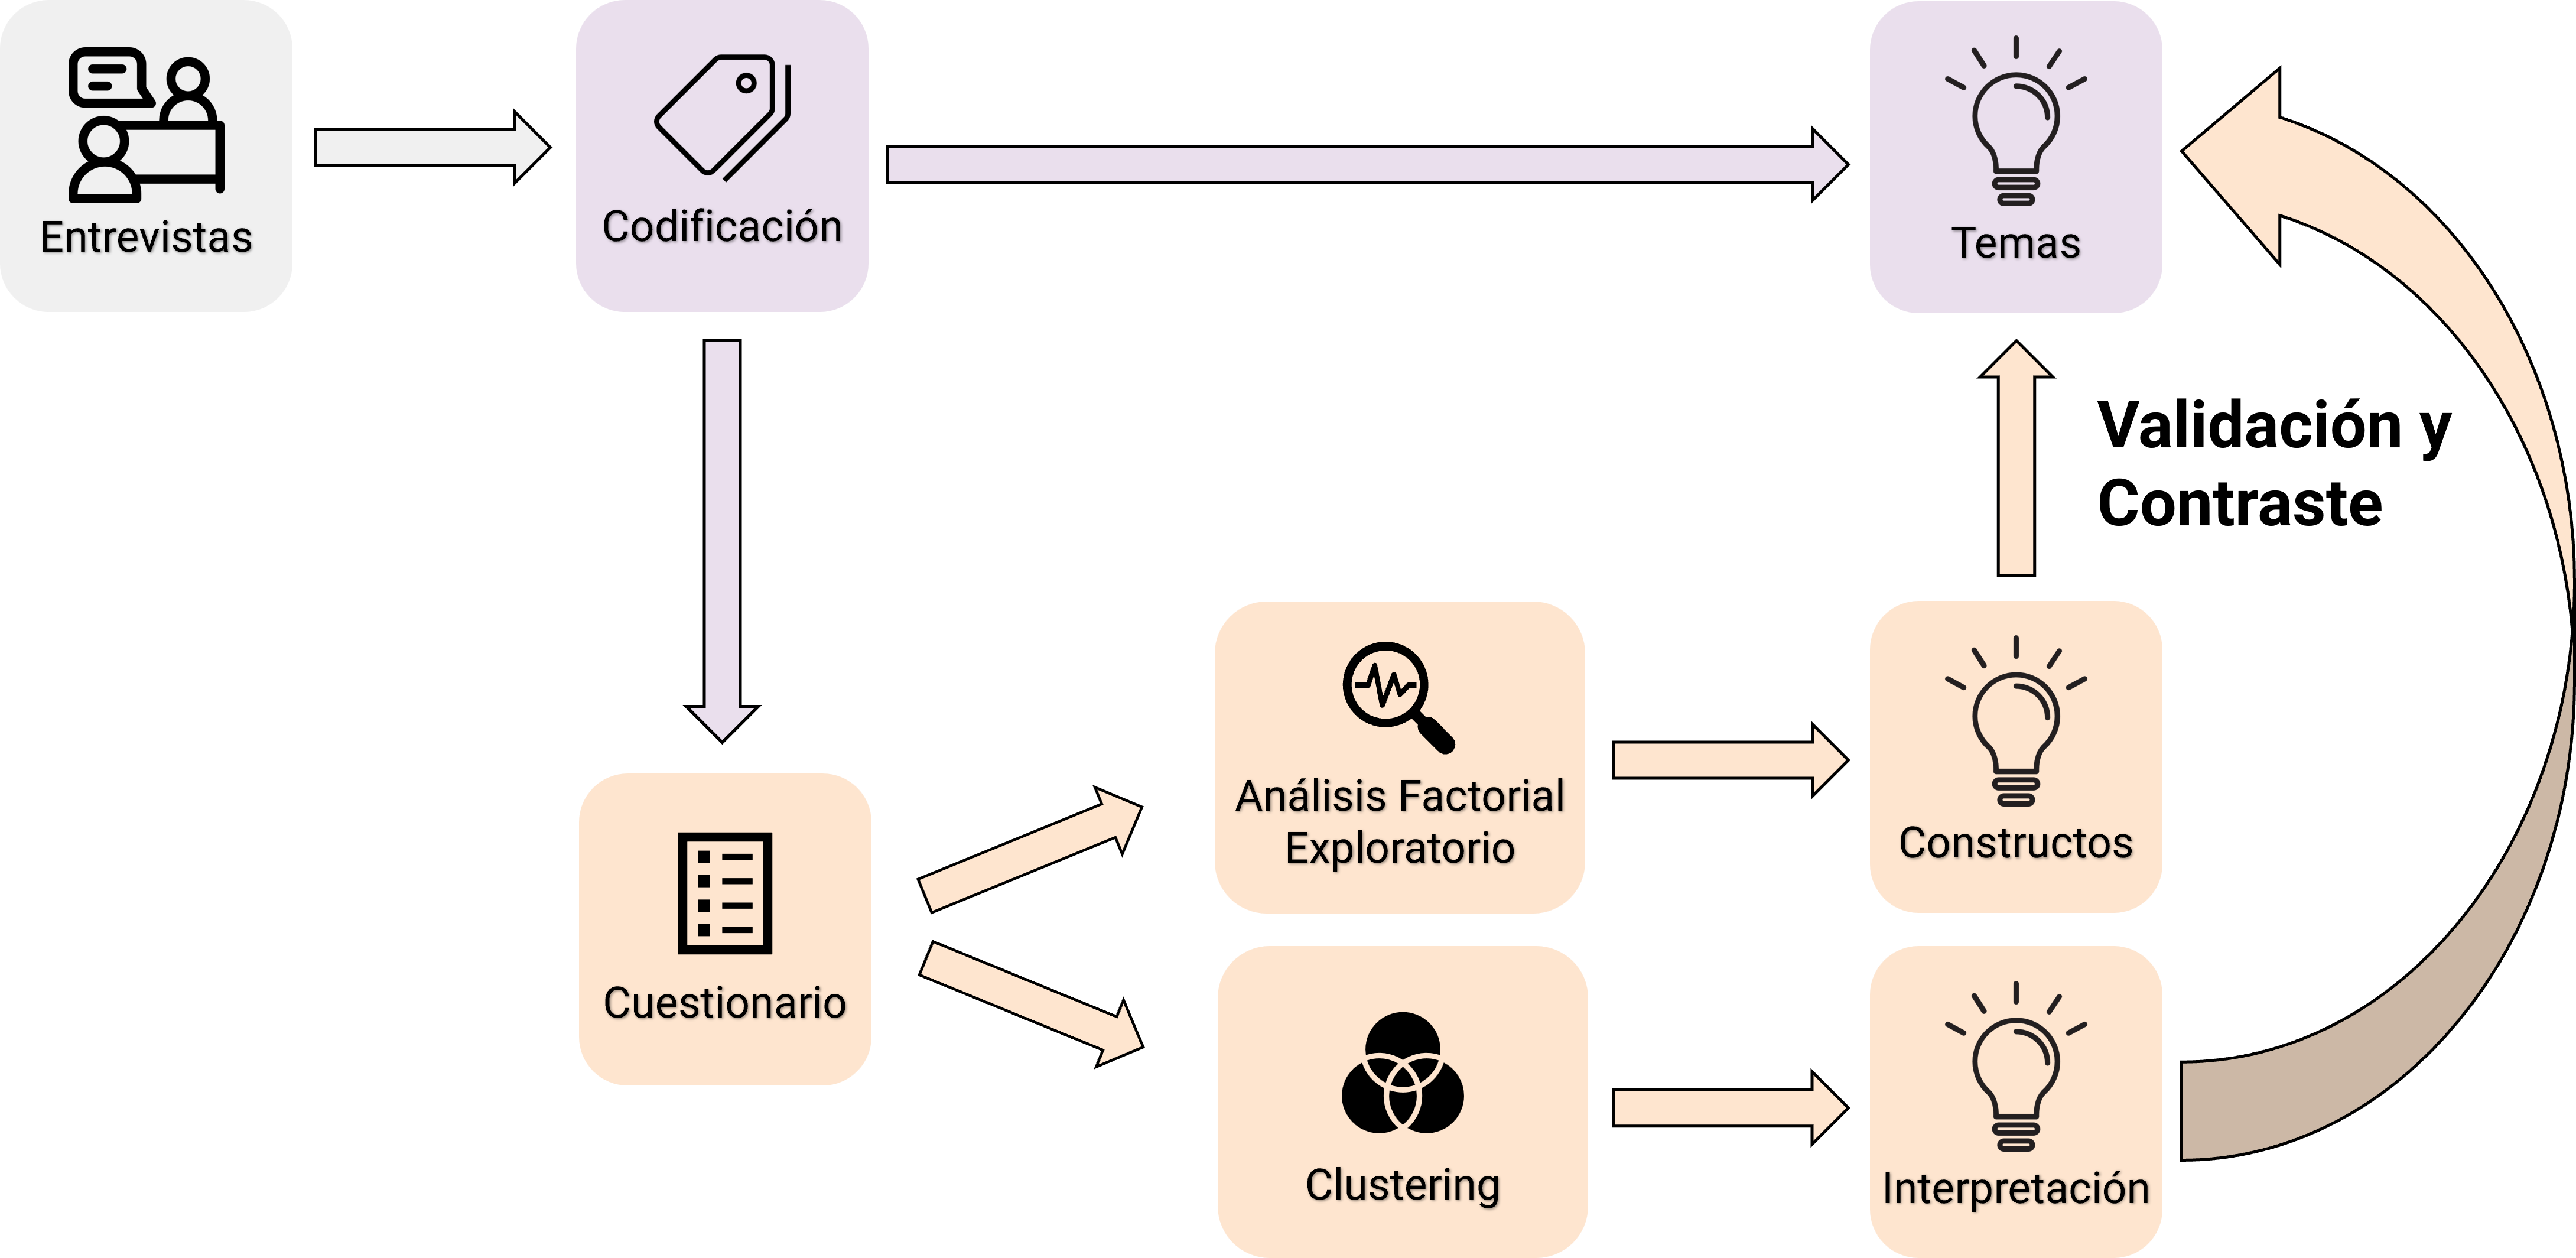
\includegraphics[width=0.5\textwidth]{img/relacion_cuali_cuanti.png}
    \caption{Proceso de validación y contraste de los temas cualitativos originalmente planteados.}
    \label{fig:relacion_cuali_cuanti}
\end{figure}

Como puede observarse, el modelo identifica dos variables latentes relacionadas con las emociones, una asociada a las emociones positivas y otra a las emociones negativas. Este patrón coincide con los resultados del análisis bivariado y del análisis de clústeres. Al comparar estos hallazgos con la tabla~\ref{tab:temas_codigos}, que presenta las codificaciones originales del estudio cualitativo, se evidencia que el análisis cuantitativo logró distinguir ambos tipos de emociones, a pesar de la alta prevalencia de emociones negativas. En consecuencia, estos resultados respaldan la conveniencia de desagregar el código original de emociones en dos categorías diferenciadas.

Asimismo, el modelo confirma la existencia del tema 2, correspondiente a la distracción. Este resultado también es consistente con el clúster 2, denominado \textit{Sobrecargados por cuidados}, ya que en este grupo se concentran principalmente los estudiantes que indicaron que el cuidado de personas dependientes fue uno de los principales factores de distracción durante las clases virtuales. Es importante señalar que este constructo se identifica a partir de un código asociado originalmente con otro tema cualitativo, como se muestra en la figura \ref{fig:relacion_codigos_sem}. Esto sugiere que, aunque el constructo está claramente definido en los resultados cualitativos y cuantitativos, el código \textit{desafíos de aprendizaje} podría estar capturando más de un constructo, no corresponder al tema en el que fue inicialmente clasificado o presentar una codificación inadecuada.

\begin{figure*}[!htb]
    \centering
    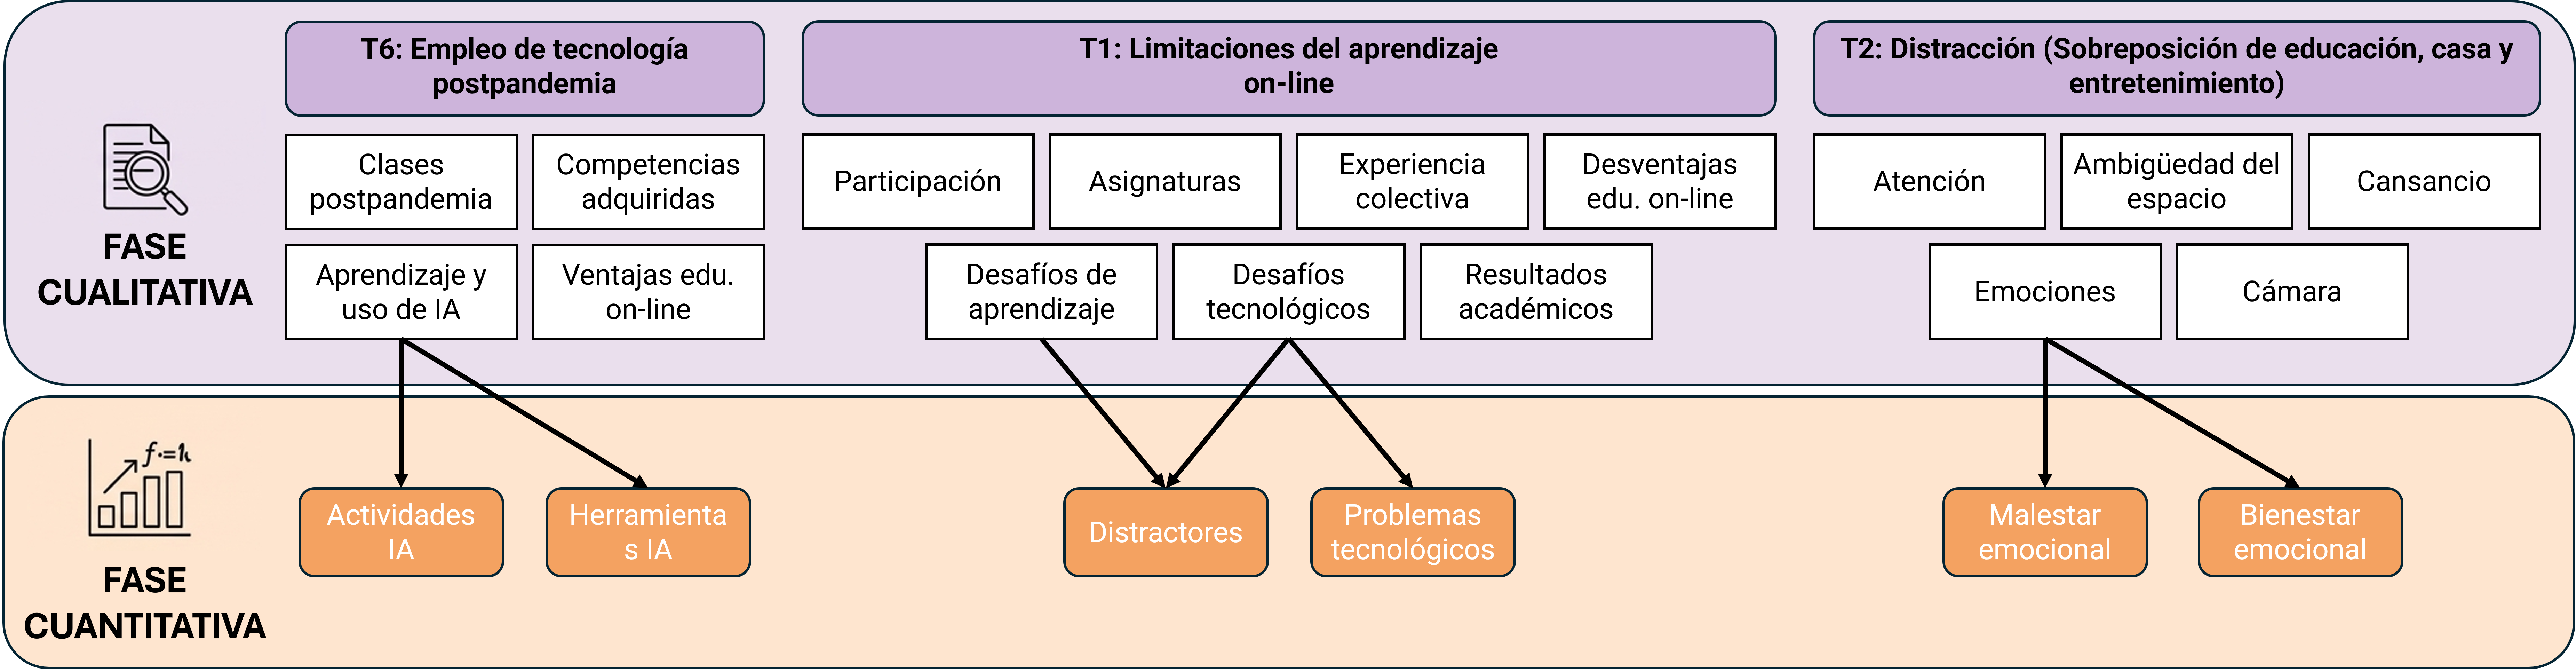
\includegraphics[width=\textwidth]{img/relacion_codigos_sem.png}
    \caption{Relación entre los constructos identificados mediante el modelo SEM y los códigos y temas propuestos inicialmente en el análisis cualitativo.}
    \label{fig:relacion_codigos_sem}
\end{figure*}


Por otra parte, la variable latente \textit{Problemas tecnológicos} está conformada por los problemas técnicos y las dificultades de conexión a Internet que llevaron a los estudiantes a apagar la cámara. Esta asociación es consistente con los resultados presentados en la tabla~\ref{tab:bivariado} y guarda relación con los clústeres 1 y 2, en los que se concentran estudiantes con dificultades técnicas. En este sentido, los resultados sugieren que los problemas tecnológicos podrían constituir un subtema representativo del tema 1 (\textit{Limitaciones del aprendizaje on-line}).

Finalmente, el modelo sugiere desagregar el código \textit{uso de IA} en dos constructos diferenciados. El primero hace referencia a las distintas herramientas de inteligencia artificial que los estudiantes utilizan tras el retorno a la presencialidad, mientras que el segundo representa los diferentes usos que hacen de dichas herramientas. Aunque esto no se evidenció en los análisis cuantitativos previos, resulta razonable considerar que existe una distinción relevante entre el uso y la selección de herramientas de IA, dado que algunas de ellas tienen fines específicos.

\vspace{0.5em}
\noindent\textbf{Análisis Factorial Confirmatorio}

El CFA se aplicó a cada uno de los modelos SEM evaluados con el objetivo de analizar la estabilidad de los resultados bajo diferentes supuestos distribucionales. Para ello, se emplearon múltiples estimadores, incluyendo MLW (\textit{Maximum Likelihood with Welch correction}), basado en máxima verosimilitud robusta; DWLS (\textit{Diagonally Weighted Least Squares}), adecuado para datos ordinales y distribuciones alejadas de la normalidad; WLS (\textit{Weighted Least Squares}) y ULS (\textit{Unweighted Least Squares}), basados en mínimos cuadrados ponderados y no ponderados, respectivamente; así como sus variantes robustas WLSMV y MLR, orientadas al tratamiento de datos categóricos y no normales. Adicionalmente, se exploró una especificación basada en correlaciones policóricas utilizando el estimador WLSMV \cite{kline2023principles}. 

El ajuste de los modelos se evaluó mediante diferentes índices complementarios. El CFI (\textit{Comparative Fit Index}) permitió medir la mejora proporcional del ajuste del modelo respecto a un modelo base, mientras que el TLI proporcionó una evaluación similar incorporando una penalización asociada a la falta de parsimonia o al exceso de complejidad del modelo. Por otro lado, el RMSEA permitió estimar el error de aproximación poblacional considerando los grados de libertad del modelo, mientras que el SRMR cuantificó la magnitud promedio de las discrepancias entre las correlaciones observadas y las estimadas por el modelo \cite{kline2023principles}.

Los resultados de la evaluación del ajuste de los diez modelos SEM considerados en el estudio se presentan en la tabla~\ref{tab:indices_ajuste}, donde se resumen los índices de bondad de ajuste obtenidos, excluyendo aquellos con rendimientos menores y aquellos que no lograron la convergencia del modelo. En general, los resultados evidencian diferencias importantes entre las especificaciones evaluadas, destacando el impacto de la estructura propuesta y del tipo de matriz de correlación utilizada. Cabe señalar que tanto DeepSeek como Gemini fueron consultados mediante el mismo \textit{prompt} (Anexo~\ref{sec:anexo_prompt}) para mantener un criterio homogéneo. Bajo este esquema, los modelos generados por DeepSeek presentaron el mejor desempeño global, alcanzando un ajuste óptimo tanto en la versión agrupada como en la desagregada mediante matriz de Pearson, con valores de $\text{CFI} = 0.9953$ y $\text{RMSEA} = 0.0177$, lo que indica una adecuada correspondencia entre la estructura propuesta y los datos observados. Por su parte, el modelo original y el segundo derivado alcanzaron un ajuste sobresaliente únicamente en sus versiones desagregadas con matriz policórica ($\text{CFI} = 0.9739$, $\text{TLI} = 0.9730$), sugiriendo que la consideración de la naturaleza ordinal de los indicadores permite representar mejor las relaciones entre variables observadas y constructos latentes, respaldando el modelo de medición planteado inicialmente en la parte cualitativa del estudio. En contraste, los modelos generados por Gemini no mostraron un ajuste estructural adecuado; aunque presentaron valores aceptables de CFI con matriz Pearson, el elevado error de aproximación ($\text{RMSEA} = 0.1891$) evidencia limitaciones importantes en su capacidad para reproducir la estructura de relaciones presente en los datos.

\begin{table*}[!htb]
\centering
\footnotesize
\begin{tabular}{p{1.5cm}p{2.5cm}p{2.2cm}p{1.5cm}ccccc}
\toprule
\textbf{Matriz} & \textbf{Modelo} & \textbf{Versión} & \textbf{Estimador} & 
\textbf{CFI} & \textbf{TLI} & \textbf{RMSEA} & \textbf{SRMR} \\
\midrule
Pearson & DeepSeek & Agrupada & DWLS & 0.9953 & 0.9918 & 0.0177 & 0.0370 \\
Pearson & DeepSeek & Desagregada & DWLS & 0.9018 & 0.8940 & 0.0451 & 0.0629 \\
Pearson & Gemini & Agrupada & ULS & 0.8977 & 0.8706 & 0.1891 & 0.1124 \\
Pearson & Gemini & Desagregada & DWLS & 0.8458 & 0.8350 & 0.0493 & 0.0667 \\
Pearson & Original & Agrupada & DWLS & 0.7768 & 0.7455 & 0.0425 & 0.0596 \\
Pearson & Original & Desagregada & DWLS & 0.6807 & 0.6701 & 0.0463 & 0.0686 \\
Pearson & Primer derivado & Agrupada & ULS & 0.8773 & 0.8558 & 0.1437 & 0.0675 \\
Pearson & Primer derivado & Desagregada & DWLS & 0.7973 & 0.7897 & 0.0382 & 0.0640 \\
Pearson & Segundo derivado & Agrupada & DWLS & 0.7770 & 0.7457 & 0.0425 & 0.0596 \\
Pearson & Segundo derivado & Desagregada & DWLS & 0.6852 & 0.6747 & 0.0460 & 0.0683 \\
\midrule
Policórica & DeepSeek & Agrupada & MLR & 0.9794 & 0.9644 & 0.0374 & 0.0365 \\
Policórica & Gemini & Agrupada & MLR & 0.6965 & 0.5930 & 0.0854 & 0.1029 \\
Policórica & Original & Desagregada & WLSMV & 0.9739 & 0.9730 & 0.0558 & 0.1256 \\
Policórica & Primer derivado & Agrupada & MLR & 0.7948 & 0.7587 & 0.0422 & 0.0566 \\
Policórica & Primer derivado & Desagregada & WLSMV & 0.7815 & 0.7733 & 0.0498 & 0.1145 \\
Policórica & Segundo derivado & Desagregada & WLSMV & 0.9739 & 0.9730 & 0.0558 & 0.1256 \\
\bottomrule
\end{tabular}
\caption{Métricas de ajuste de las mejores versiones de los modelos SEM.}
\label{tab:indices_ajuste}
\end{table*}

El excelente ajuste del modelo DeepSeek con datos agrupados ($\text{CFI} = 0.9953$, $\text{RMSEA} = 0.0177$) sugiere que la estructura de cuatro variables latentes propuesta por este LLM captura de manera parsimoniosa y precisa las relaciones subyacentes en los datos. La superioridad de este modelo sobre el Original ($\text{CFI} = 0.7768$) y sus derivados evidencia que la integración de resultados de AFE con la capacidad inferencial de los LLM puede superar las especificaciones basadas únicamente en el marco cualitativo.

El buen ajuste del modelo Original en su versión desagregada con matriz policórica ($\text{CFI} = 0.9739$) es particularmente relevante porque valida la estructura de constructos derivada exclusivamente del análisis cualitativo, pero únicamente cuando se respeta la naturaleza ordinal de los datos mediante el uso de correlaciones policóricas. Esto sugiere que el marco cualitativo original es conceptualmente sólido, pero su operacionalización cuantitativa requiere considerar adecuadamente la escala de medición de los indicadores.

Por el contrario, el pobre desempeño de los modelos Gemini, a pesar de su alta fiabilidad (tabla~\ref{tab:fiabilidad}), indica que la consistencia interna de los constructos no garantiza un buen ajuste estructural. Esto refuerza la importancia de evaluar los modelos SEM tanto desde la perspectiva de la fiabilidad como del ajuste global, ya que un modelo puede tener constructos bien medidos, pero relaciones estructurales mal especificadas.

\subsection{Fiabilidad de los modelos SEM}

La tabla~\ref{tab:fiabilidad} resume los promedios de las métricas de consistencia interna a lo largo de las variables latentes de cada modelo SEM. Se evidencia una clara limitación en el Alfa de Cronbach, el cual presenta estimaciones deficientes en todos los casos e incluso valores negativos en las versiones agrupadas, lo que confirma la invalidez del supuesto de tau-equivalencia en estos datos debido a que no todas las preguntas se encontraban en una misma escala de medición. En contraste, los indicadores robustos de omega de McDonald ($\Omega$) y fiabilidad compuesta ($\mathrm{CR}$) muestran un comportamiento óptimo y convergente entre sí. Bajo estas métricas, los modelos DeepSeek y Gemini demuestran una alta fiabilidad en la medición ($\Omega / \mathrm{CR} \geq 0.8017$), superando al modelo Original y sus variantes derivadas, los cuales únicamente alcanzan niveles de consistencia aceptables en su modalidad desagregada ($\Omega / \mathrm{CR} \approx 0.73$). Aun así, estos resultados indican que el modelo propuesto en la parte cualitativa sí presenta una fiabilidad estadística aceptable para el conjunto de datos desagregado.

\begin{table*}[!htb]
\centering
\footnotesize
\begin{tabular}{p{2.8cm}p{2.2cm}cccc}
\toprule
\textbf{Modelo} & \textbf{Dataset} & \textbf{Variables latentes} & 
\textbf{Prom. Cronbach} & \textbf{Prom. Omega McDonald} & \textbf{Prom. CR} \\
\midrule
DeepSeek & Agrupada & 4 & -0.0033 & 0.8200 & 0.8200 \\
DeepSeek & Desagregada & 6 & 0.4089 & 0.8250 & 0.8250 \\
Gemini & Agrupada & 4 & -0.0033 & 0.8200 & 0.8200 \\
Gemini & Desagregada & 18 & 0.2186 & 0.8017 & 0.8017 \\
Original & Agrupada & 6 & 0.2168 & 0.6193 & 0.6193 \\
Original & Desagregada & 6 & 0.5335 & 0.7274 & 0.7274 \\
Primer derivado & Agrupada & 6 & 0.2109 & 0.6276 & 0.6276 \\
Primer derivado & Desagregada & 6 & 0.5768 & 0.7298 & 0.7298 \\
Segundo derivado & Agrupada & 6 & 0.2168 & 0.6193 & 0.6193 \\
Segundo derivado & Desagregada & 6 & 0.5335 & 0.7274 & 0.7274 \\
\bottomrule
\end{tabular}
\caption{Métricas promedio de fiabilidad de cada modelo SEM.}
\label{tab:fiabilidad}
\end{table*}

Los modelos generados por IA superan en fiabilidad media al modelo original y sus derivados, aunque solo DeepSeek logra traducir esa fiabilidad en un buen ajuste confirmatorio. La discrepancia entre la alta fiabilidad del modelo Gemini agrupado y su pobre ajuste sugiere que sus constructos, aunque internamente consistentes, no se relacionan entre sí de la forma especificada en el modelo estructural. Esto subraya la necesidad de evaluar los modelos SEM de manera integral, considerando tanto la fiabilidad de los constructos como la validez estructural de las relaciones propuestas.

La deficiencia sistemática del Alfa de Cronbach, especialmente en las versiones agrupadas donde alcanza valores negativos, confirma las advertencias de la literatura sobre su inadecuación cuando los ítems no son tau-equivalentes \cite{mcdonald1999test}. Este hallazgo tiene implicaciones metodológicas importantes para futuros estudios que utilicen escalas heterogéneas, por lo que se recomienda el uso del omega de McDonald o de la fiabilidad compuesta como indicadores primarios de consistencia interna.

% \section{Formalización del proceso de validación}
% \label{sec:formalizacion}

% A fin de sintetizar el procedimiento descrito y dotarlo de un carácter reproducible, el proceso de validación de constructos se formaliza mediante teoría de conjuntos. Se definen el conjunto de temas cualitativos $T$, el de códigos $C$, el de técnicas de reducción de dimensionalidad $\mathcal{R}$, el de algoritmos de clustering $\mathcal{A}$, el de estimadores $\mathcal{E}$ y el de matrices de correlación $\mathcal{C}$. La entrada del proceso la constituyen los datos brutos $D_{raw}$ y el marco cualitativo $\{T, C\}$, mientras que la salida corresponde al modelo óptimo $M^*$, la partición $P^*$ y la interpretación $\text{Interp}$ de los perfiles. El algoritmo 1 consolida las etapas de limpieza, análisis exploratorio, división de los datos en las versiones desagregada ($D_z$) y agrupada ($D_{agg}$), y los dos flujos paralelos de clustering y de especificación estructural.

% El algoritmo opera en cuatro fases, seguidas de una etapa final de selección. La primera depura los datos brutos y ejecuta el análisis exploratorio univariado y bivariado, del que se obtienen los estadísticos $E_U$ y las asociaciones $A_B$. La segunda estandariza el conjunto limpio y, mediante agregación por constructo guiada por los códigos $C$, genera las versiones $D_z$ y $D_{agg}$. La tercera y la cuarta corresponden a dos flujos en paralelo: el flujo de clustering explora varias combinaciones de reducción de dimensionalidad $r \in \mathcal{R}$ y algoritmos $a \in \mathcal{A}$ con sus hiperparámetros $\theta$, evaluando cada partición mediante los índices de Silhouette ($S$), Davies-Bouldin ($DB$) y Calinski-Harabasz ($CH$), para que el modelo de lenguaje seleccione la partición óptima $P^*$ e interprete los perfiles; el flujo factorial, por su parte, aplica el filtrado iterativo por KMO y MSA, la prueba de esfericidad de Bartlett y el análisis de componentes principales con rotación Varimax, obteniendo la matriz de cargas $L_{rot}$ a partir de la cual el modelo de lenguaje propone el modelo $M_{SEM}$. Finalmente, la etapa de AFC evalúa cada especificación sobre las matrices de correlación $\mathcal{C}$ y los estimadores $\mathcal{E}$, reteniendo como óptimo el modelo que supere los umbrales $\tau_{CFI}$, $\tau_{RMSEA}$ y $\tau_{\Omega}$ y que maximice las métricas correspondientes.

% % ============================================================  

\section{Conclusiones y trabajo futuro}
\label{sec:conclusiones}
% ============================================================

Este estudio aplicó métodos mixtos con el fin de articular los hallazgos cualitativos con los cuantitativos en un diseño secuencial exploratorio orientado a analizar la experiencia estudiantil en la educación virtual postpandemia en la Universidad de Cuenca. A partir de un marco cualitativo de seis temas, se construyó un cuestionario aplicado a 513 estudiantes y se integraron análisis exploratorio, clustering, análisis factorial exploratorio y modelos de ecuaciones estructurales generados con apoyo de inteligencia artificial. El modelo inferido por DeepSeek con datos agrupados alcanzó un ajuste excelente en el análisis confirmatorio, superando al modelo original y al resto de especificaciones, lo que evidencia que los grandes modelos de lenguaje, cuando se nutren de resultados factoriales y teoría, pueden proponer estructuras latentes coherentes y empíricamente sólidas.

Los análisis cuantitativos confirmaron la bidimensionalidad de las emociones vividas en la virtualidad, diferenciando un polo negativo (estrés, ansiedad, monotonía, depresión) de un polo positivo (gratitud, confianza, proactividad), patrón que se replicó en asociaciones bivariadas, perfiles de clustering y en el modelo desagregado de DeepSeek. Asimismo, emergió un factor de distracción asociado al cuidado de dependientes, y se identificó que los problemas técnicos constituyen un subcomponente relevante dentro de las limitaciones del aprendizaje en línea. Respecto al uso de inteligencia artificial, los resultados aconsejan desagregar su medición en dos constructos: la selección de herramientas y las actividades específicas realizadas con ellas.

En el plano de la fiabilidad, los modelos generados por inteligencia artificial mostraron un omega de McDonald y una fiabilidad compuesta superiores en comparación con el modelo original y sus versiones derivadas. Además, este resultado evidencia las limitaciones del alfa de Cronbach ante escalas heterogéneas y confirma la idoneidad de indicadores más robustos. El trabajo demuestra que la transición trazable desde códigos cualitativos hasta constructos cuantitativos, mediada por técnicas multivariadas y el apoyo de IA, permite operacionalizar la integración auténtica entre métodos, a la vez que posibilita refinar el marco interpretativo de partida. Entre las limitaciones destacan la unicidad institucional de la muestra y el carácter transversal de los datos; las líneas futuras podrían replicar el proceso desarrollado en otras poblaciones, implementar estudios longitudinales y formalizar la retroalimentación cuantitativa hacia la revisión de los temas cualitativos, cerrando el ciclo integrador propio de los métodos mixtos.

% ============================================================
% BIBLIOGRAFÍA
% ============================================================

\bibliographystyle{IEEEtran}
\bibliography{referencias}

% ============================================================
% ANEXOS
% ============================================================

\appendices
\section{Directiva de Prompting para Modelos SEM}
\label{sec:anexo_prompt}

El siguiente \textit{prompt} se utilizó para generar los modelos SEM teóricos mediante LLM:

\begin{quote}
\footnotesize
\noindent\textbf{Rol y contexto:} \textit{«Actúa como un investigador experto en psicometría y Modelado de Ecuaciones Estructurales (SEM). Se te proporcionan los resultados del Análisis Factorial Exploratorio (AFE) tras preprocesamiento (filtrado iterativo KMO y MSA individual $\ge 0.70$, extracción PCA con al menos el 80\% de varianza acumulada explicada y matriz rotada de cargas factoriales Varimax), acompañados del diccionario de variables del instrumento.»}

\vspace{0.3em}
\noindent\textbf{Instrucciones de análisis:} \textit{«Analiza cada archivo de manera independiente (para la versión desagregada y la agrupada) y ejecuta las siguientes tareas:
\begin{enumerate}
    \item \textbf{Definición de constructos:} Identifica y define las variables latentes a partir de las agrupaciones de variables observadas en la matriz rotada Varimax.
    \item \textbf{Fundamentación teórica:} Propón las relaciones estructurales y correlaciones direccionales entre las variables latentes identificadas, justificando conceptualmente cada vínculo a partir de literatura científica sobre educación virtual (indicando las referencias y fuentes de respaldo).
    \item \textbf{Especificación formal:} Formula el modelo de medición y el modelo estructural en sintaxis estándar de SEM para Python (formato tipo lavaan: \texttt{latente =\textasciitilde{} manifiesta1 + manifiesta2}).»
\end{enumerate}}
\end{quote}

\end{document}
